\subsection{Bayesian Inference}
The Bayesian inversion approach samples a posterior distribution of depth profiles. For comparison to the other inversion methods, we consider only the depth at each grid point which corresponds to the maximum of the posterior probability distribution at that point. This is achieved by taking the maximum of the kernel density of the estimated depth distribution at each point along the 1D profile. 

This method is first applied using synthetic $k$ input and the resulting depth estimate is shown in Figure~\ref{mcmc-synthetic}. As for other methods, the synthetic result accurately represents the sandbar located at $x~\sim~950~m$ along the profile, which is an important feature to recreate. However, at offshore locations ($x~<~600~m$), the estimation appears to break down. As in other methods, this is expected because of the lower sensitivity of $k$ on $h$ at these depths, a relationship on which our inverse methods rely.

\begin{figure}[H]
\center
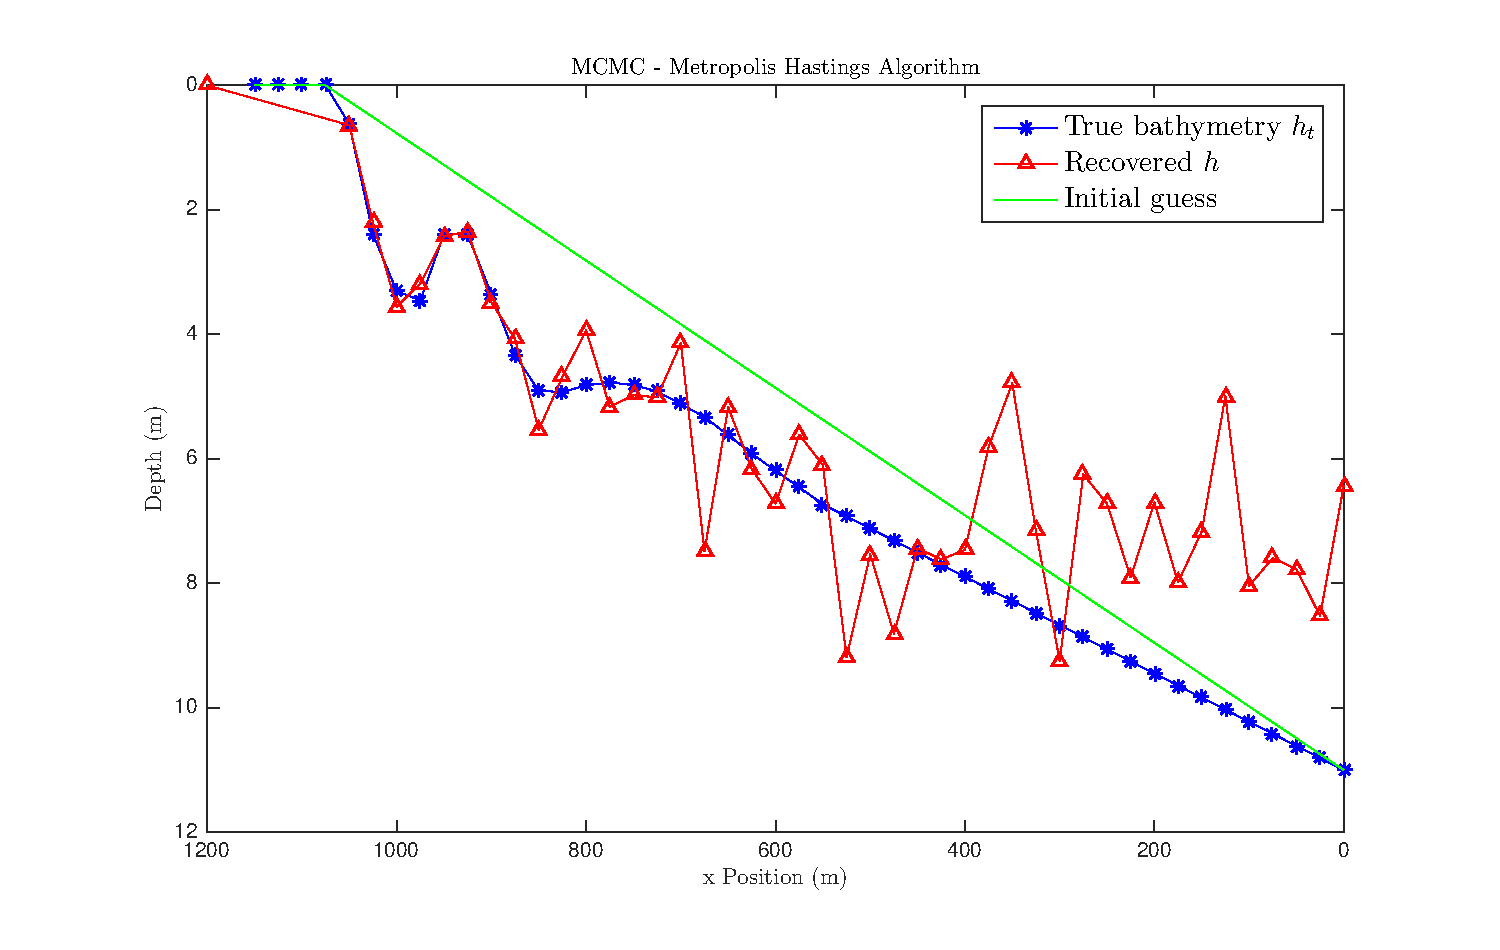
\includegraphics[scale=0.46]{img/MCMC-manufactured.eps} 
\caption{Bathymetry estimate from the Bayesian Markov Chain Monte Carlo approach. The initial $h$ guess is shown in green, the true $h$ is shown in blue, and the derived estimate of $h$ is shown in red.}
\label{mcmc-synthetic}
\end{figure}

The synthetic data MCMC results were generated using 20,000 iterations of the Metropolis algorithm after 1000 ``burn in" iterations were discarded. The first iterations are considered to be a transient and unreliable portion of the solution so extra iterations, known as ``burn in" iterations are included to account for this. Proposal $h_{i+1}$ profiles were computed by adding a randomly generated step to $h_i$ and a proposal posterior distribution was computed for the $(i+1)th$ step. An arbitrary scale factor of 0.5 was used to moderate the step size between iterations. 

\begin{figure}[H]
\center
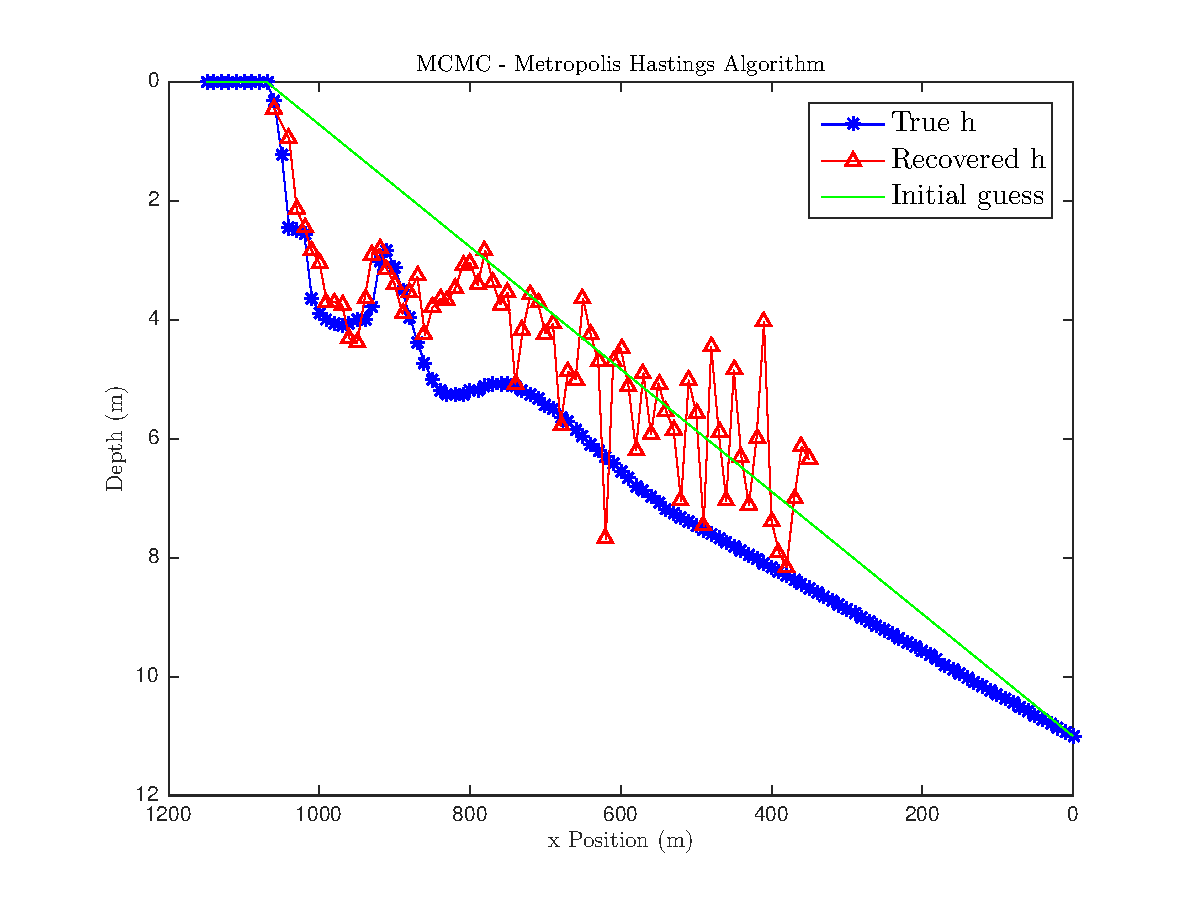
\includegraphics[scale=0.46]{img/REAL_plot1_chopped_propSD0_1prSD0_5_totstep1000_kOct9.eps}
\caption{Bathymetry estimate from the Bayesian Markov Chain Monte Carlo approach using measured wave numbers as the objective in the likelihood function. The initial $h$ guess is shown in green, the true $h$ is shown in blue, and the derived estimate of $h$ is shown in red.}
\label{mcmc-real}
\end{figure}

Real $k$ data is used to estimate the same bathymetry profile (Figure~\ref{mcmc-real}). As with the synthetic case, we find a good match to the sandbar region around $x\sim900~m$. However, the estimated depth decreases just seaward of the sand bar and does not correlate well with the true bathymetry for the remainder of the seaward domain. We expectt the noisy spike in $k$ seaward of the sandbar seen in  Figure~\ref{effectivewavenumbernoise} may be responsible for errors in our estimate of $h$ in this area. The same issue occurs in the other inversion depth estimates. Note observed values of $k$ are unavailable seaward of $\sim350~m$, so we do not estimate a depth for this region. 

Overall, the MCMC result performs better for the synthetic case, as may be expected given increased noise in real observations of $k$. We compute this depth estimate using 1000 iterations with 250 burn in iterations and a proposal step size of 0.1. It it possible that inclusion of the wave height, $H$, as an additional objective in the likelihood function would improve estimates seaward of the sandbar where $k$ becomes less sensitive to depth, $h$, however we have yet to test this with the MCMC method. We also expect that additional scrutiny of our choices for the prior, proposal step size, and number of iterations could result in an improved bathymetry estimate given observed wave number, $k$. 

Unlike the other methods, the Bayesian approach results in a distribution of depth profiles which optimize $h$ given uncertain $k$. Measurements of wave number, $k$, are not perfect and our resulting distribution of depth profiles translates that uncertainty binto an ensemble of depth estimates which are consistent with the $k$ data to within uncertainty. Figures~\ref{mcmc-posterior-h-synthetic} and \ref{mcmc-posterior-h-real} show the resulting posterior depth distributions. Note that...






